%-----------------------------------------------------------------
%	AGRUPACIONS DE GALÀXIES
%	!TEX root = ./../main.tex
%-----------------------------------------------------------------
\section{Agrupacions de galàxies}\label{sec:galaxies}
\subsection{Classificació de les galàxies}
Les galàxies solen classificar-se atenent al seu aspecte en la longitud d'ona del visible.

El tipus més abundant de galàxia és el de nana poc lluminosa; les galàxies grans i les gegants emeten una enorme quantitat de llum.

L'existència de galàxies (més enllà de la Via Làctia) va ser establida als anys 20. Abans d'això, apareixien als catàlegs com a «nebuloses», sistemes lluminosos, suposadament dins els confins de la Galàxia. En les imatges captades pels telescopis les nebuloses apareixien borroses i per tant es creia que eren mancants d'estrelles.
\begin{figure}[h]
	\centering
	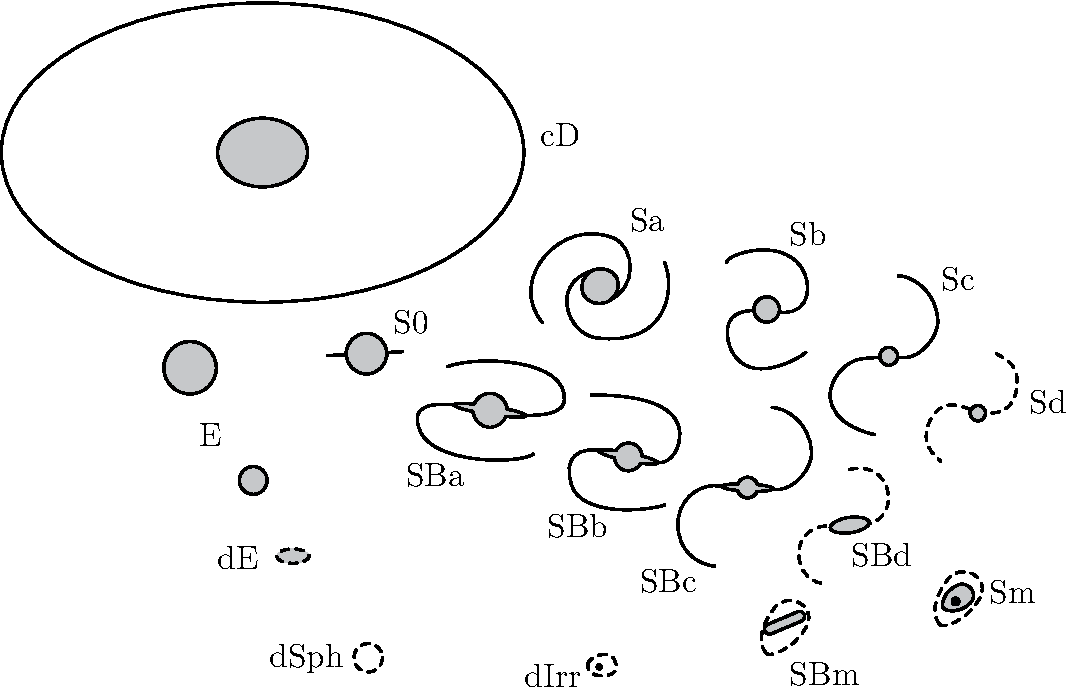
\includegraphics[width=0.8\textwidth]{./images/8-hubble-scheme}
	\caption{Esquema original de Hubble amb certes modificacions}
	\label{fig:hubble-scheme}
\end{figure}

Hubble, amb l'ajut del telescopi del \textit{Mount Wilson Observatory} (MWO), va trobar estrelles variables a la «nebulosa» M31 (Andròmeda) [\href{http://apod.nasa.gov/apod/ap130626.html}{APOD~130626}], i va advertir que el ritme de variació de la llum seguia el mateix patró que les Cefeides de la Via Làctia. Sota la hipòtesi que eren estrelles del mateix tipus, va aplicar l'equació $F = L/ (4\pi d^2)$ tot trobant $d \gtrsim \SI{300}{\kilo\parsec}$ com a distància a Andròmeda; de manera que aquesta havia de ser una galàxia i no un sistema interior a la Via Làctia. Avui dia se sap que la distància a Andròmeda és aproximadament $\SI{800}{\kilo\parsec}$.

Hubble va establir a \textit{The Realm of the Nebulae} (1936) un esquema de classificació de les galàxies (figura \ref{fig:hubble-scheme}). En dit esquema hi ha tres tipus de galàxies (el·líptiques, lenticulars, i espirals) més un quart tipus (irregulars) per aquelles que no s'ajusten a cap dels tipus interiors.

%-------------------------------
\subsubsection*{Galàxies el·líptiques (E)}
Són arrodonides sense característiques especials (ni braços espirals ni franges de pols). Normalment manquen de núvols freds de gas per la qual cosa posseeixen no poques estrelles blaves joves. Un estudi detallat revela que les el·líptiques gegants posseeixen una estructura diferent de les petites i poc lluminoses. N'hi ha amb un disc dins el cos el·líptic.

Les el·líptiques predominen en cúmuls de moltes galàxies i les el·líptiques més grans (galàxies CD) solen trobar-se en la zona més densa d'aquests cúmuls. Les galàxies CD consten d'un nucli el·líptic rodejat d'una enorme i difusa embolcall que pot assolir centenars de kiloparsecs. Aquests sistemes arriben a ser fins a 100 cops més lluminosos que la Via Làctia.

Les el·líptiques de mida mitjana i gegants posseeixen una lluminositat varies vegades la de la Galàxia, i mides de l'ordre de desenes de kiloparsecs. Les seves estrelles segueixen un moviment en aparença poc organitzat i les seves òrbites en torn al centre de la galàxia estan orientades erràticament. En el·líptiques menys massives i menys lluminoses les estrelles tenen un moviment més ordenat i menys erràtic.

Les el·líptiques molt poc lluminoses ($\sim 1/10$ de la Via Làctia) solen ser de dos tipus:
\begin{enumerate}[(i)]
	\item Galàxies compactes, com el sistema M32 [\href{http://apod.nasa.gov/apod/ap960106.html}{APOD~960106}].
	\item Galàxies nanes difuses (dE) [\href{http://apod.nasa.gov/apod/ap001023.html}{APOD~001023}], i les encara menys lluminoses nanes esferoïdals (dSph) [\href{http://apod.nasa.gov/apod/ap990122.html}{APOD~990122}]. Aquestes últimes són a penes visibles a les plaques fotogràfiques.
\end{enumerate}

Les galàxies tipus dE i les dSph no mostren gairebé moviment de rotació.

%-------------------------------
\subsubsection*{Galàxies lenticulars (S0)}
Posseeixen un disc rotatori a més d'un cos central el·líptic, però aquest manca de braços espirals o de grans franges de pols. Poden considerar-se com un tipus intermedi entre el·líptiques i espirals. Són semblants a les el·líptiques en el fet que solen trobar-se a regions molt poblades. S'assemblen a les espirals en la presència del disc que gira ràpidament. N'és un exemple la galàxia NGC 2787 [\href{http://apod.nasa.gov/apod/ap020408.html}{APOD~020408}].

%-------------------------------
\subsubsection*{Galàxies espirals (S)}
Posseeixen braços espirals brillants en què destaca la llum blava d'estrelles joves. Els braços queden delineats per grups per grups d'estrelles O i B calents, i per núvols de gas i pols a partir de les quals es formen aquestes estrelles.

Aproximadament la meitat de les espirals i lenticulars posseeixen una barra central. Els sistemes SB0, SBA, \dots, SBd formen una seqüència paral·lela a les galàxies sense barra.

Al llarg de la seqüència Sa, \dots, Sd la protuberància central es fa menys important amb respecte al disc (que gira ràpidament) i els braços s'obren més i més; i la proporció de gas i estrelles joves al disc augmenta. La Via Làctia és una Sc i potser una Sbc. Andròmeda (M31) és una Sb. En mitjana, galàxies Sc i Sd són menys lluminoses que les Sa i Sb, però algunes Sc són més brillants que una Sa típica.

Cap al final de les seqüències de galàxies espirals, Sd i SBd, els braços apareixen menys ordenats i discontinus (a trossos). Les Sm i SBm són les espirals de Magalhães (el prototip de les quals és LMC, el Gran Núvol de Magalhães [\href{http://apod.nasa.gov/apod/ap130528.html}{APOD~130528}]). En aquestes, l'espiral es redueix a un únic i ample braç. Conforme la lluminositat de la galàxia decreix, la velocitat de rotació del disc disminueix. Les galàxies menys brillants són menys massives. El Gran Núvol de Magalhães gira només a $\SI{80}{\km \per\s}$, un terç de la velocitat de rotació de la Via Làctia.

El moviment estel·lar erràtic també disminueix en les galàxies petites, però, tot i així, el moviment rotacional ordenat forma una part menys important de la seva energia total.

%-------------------------------
\subsubsection*{Galàxies irregulars (Irr)}
Hubble va situar en aquest grup totes aquelles galàxies que no s'ajusten a cap dels tres tipus anteriors.

Avui dia s'utilitza el nom d'\textit{irregular} només per a galàxies blaves, petites mancants de braços espirals o de qualsevol altra estructura organitzada. Les nanes irregulars es diferencien de les nanes esferoïdals en el fet que posseeixen fas i estrelles joves blaves. És possible que les nanes esferoïdals no siguin més que nanes irregulars que han esgotat o perdut gairebé tot el seu gas.

\subsubsection*{Catàlegs de galàxies}\label{sec:catalogues}
\begin{itemize}
	\item Charles Messier (1784) va catalogar 109 objectes, entre ells Andròmeda (M31).
	% FIXME: messier@sec:bio
	\item \textit{New General Catalogue} (John Dreyer, 1888, amb addicions al 1895 i al 1908), basat fonamentalment en el treball de William Herschel, conté més de 7000 objectes lluminosos com ara cúmuls d'estrelles, núvols gasosos, i galàxies. Andròmeda és NGC~224.
	% FIXME: herschel@sec:bio
	\item El catàleg de la NASA \textit{Extragalactic Database} és accessible via web: \url{https://ned.ipac.caltech.edu/}.
	\item \textit{David Dunlap Observatory Catalogue}, conegut com a DDO o \textit{A Catalogue of Dwarf Galaxies}, és un catàleg de galàxies nanes que va ser publicat al 1959 (amb addicions al 1966) per Sidney van den Bergh (1929).
\end{itemize}

%-----------------------------------------------------------------
\subsection{Fotometria galàctica}
Les galàxies no apareixen com punts de llum (cas de les estrelles) sinó com objectes extensos i borrosos sobre el fons fosc del cel nocturn (l'observació òptica de les galàxies requereix un cel sense lluna o lluna nova). La turbulència de l'atmosfera ocasiona que les galàxies apareguin borroses, i que els telescopis terrestres no puguin distingit detalls per baix de $\SI{1/3}{\arcsecond}$.

Interessa conèixer quanta llum és emesa a diferents longituds d'ona per les diferents regions de la galàxia sota observació. Per fer-ho es defineix la lluminositat superficial.

\begin{defi}[Lluminositat superficial, $I(\va{x})$]
	Es defineix la lluminositat superficial, $I(\va{x})$, com la quantitat de llum per segon d'arc quadrat sobre el cel en un punt $\va{x}$ de la imatge.

	Sigui un petit quadrat de costat $D$ a la imatge d'una galàxia que es troba a una distància $d$, de manera que aquest quadrat subtendeix un angle $\alpha = D/d$ al cel, llavors
	\begin{align}\label{eq:llum-sup}
		I(\va{x}) \equiv \frac{F}{\alpha^{2}} = \frac{L}{4\pi D^{2}}
	\end{align}
	on $L$ és la lluminositat del quadrat en qüestió.

	En un principi $I(\va{x})$ no depèn de la distància a la galàxia, no obstant, si la distància és molt gran, l'efecte d'expansió de l'Univers intervé a través del desplaçament $z$ cal al vermell.
\end{defi}

Els contorns $I(\va{x}) = cte$ s'anomenen \textit{isofotos}. L'equació \eqref{eq:llum-sup} mostra que la posició d'un isofoto en una galàxia és independent d'aquest observador.

La lluminositat superficial sol ser mesurada en una banda determinada de longitud d'ona. Es centres de galàxies solen assolir només $I_{B}(\va{x}) \approx \SI{18}{^{\prime\prime-2}}$ i $I_{R}(\va{x}) \approx \SI{16}{^{\prime\prime-2}}$. Els disc estel·lars són encara menys brillants.

Ja que les galàxies manquen de fronteres ben definides per estimar la seva mida, aquesta es mesura dins un isofoto donat. Freqüentment s'agafa l'isofoto de magnitud $m = 25$ a la banda $B$ (blava), denotat com $R_{25}$. Aquest és aproximadament l'1\% de la lluminositat del cel nocturn típic. Una altra possibilitat de mesura de la mida d'una galàxia és el \textit{radi de Holmberg}, corresponent a $I_{B}(\va{x}) = \SI{26.5}{^{\prime\prime-2}}$.

Per determinar la lluminositat d'una galàxia completa es mesura l'augment de lluminositat conforme augmenta la distància des del centre de la galàxia cap a l'exterior, tot extrapolant aquest resultat per trobar el total.

La lluminositat superficial d'una galàxia espiral decau amb la distància $r$ al seu centre al llarg del semieix major segons la llei de de Vaucouleurs:
\begin{align}\label{eq:vancouleurs}
	I(r) = I_{0} \exp[-\qty(r/r_{0})^{1/4}]
\end{align}
Aquesta llei també regeix la variació de la lluminositat en la protuberància central.

La llum al disc d'una galàxia espiral varia sinusoïdalment amb l'angle azimutal. Si aquesta llum és integrada sobre un cercle per obviar l'estructura espiral, la distribució de llum al disc segueix la llei empírica
\begin{align}
	I(r) = I_{0} \exp[-r/r_{0}]
\end{align}

Mentre que $r_{0}$ varia notablement d'una galàxia espiral a una altra, $I_{0}$ varia poc, sent el seu valor de l'ordre de $\SI{2 e4}{\Lsun \per\square\lightyear}$. No obstant, s'ha trobat que la constància de $I_{0}$ no regeix per a galàxies nanes, i probablement tampoc per a les gegants.

Hi ha moltes més galàxies poc lluminoses que grans i brillants. La figura \ref{fig:nombre-galaxies} mostra el nombre de galàxies observades en funció de la seva lluminositat $L$ segons mesures de l'\textit{Observatorio de Las Campanas} (Xile). La línia contínua correspon a la funció de Schechter:
\begin{align}\label{eq:schechter}
	\Phi (L) \Delta L = n_{\star} \qty(\frac{L}{L_{\star}}) \exp[-\frac{L}{L_{\star}}] \frac{\Delta L}{L_{\star}}
\end{align}
on $L_{\star} \approx \SI{2 e10}{\Lsun}$, més o menys la lluminositat de la Via Làctia.

\begin{figure}[h]
	\centering
	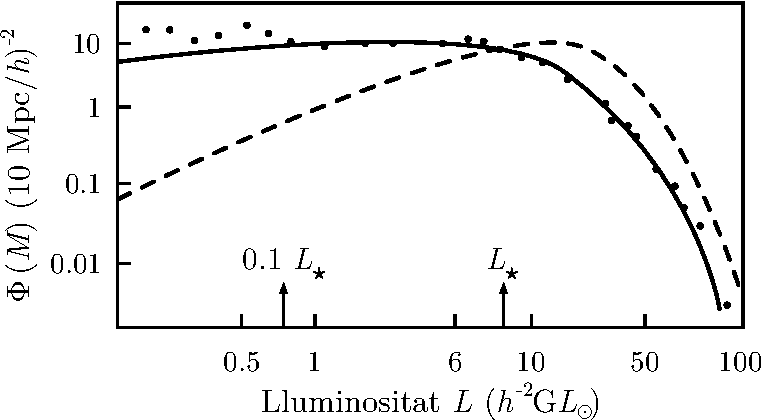
\includegraphics[width=0.6\textwidth]{./images/8-nombre-galaxies}
	\caption{Nombre de galàxies $\Phi (M)$ per a $\SI{10}{\cubic\mega\parsec}$ front a la lluminositat. La línia contínua segueix la llei de Schechter. La línia discontínua és $\Phi(M) \times L/L_{\star}$. Aquí $h \approx 0.75$ és el factor reduït de Hubble, $\alpha = -0.7$ i $n_{\star} - \SI{0.019}{\cubic\planck \per\cubic\mega\parsec}$}
	\label{fig:nombre-galaxies}
\end{figure}

A la figura \ref{fig:nombre-galaxies} s'adverteix que el nombre de galàxies en cada interval de lluminositat $\Delta L$ és quasi constant per a $L < L_{\star}$, i cau ràpidament per a $L > L_{\star}$.

La fórmula de Schechter diu que el nombre total de galàxies $\int_{0}^{\infty} \Phi (L) \dd{L}$ divergeix per a $L \to 0$. No obstant, la línia discontínua ens diu que la major part de la llum ve de les galàxies de lluminositat en torn a $L_{\star}$. La integració de la funció de Schechter ens dóna la lluminositat total:
\begin{align}
	 \int_{0}^{\infty} \Phi (L) \dd{L} = n_{\star} \Gamma (\alpha + 2) \approx \SI{1.4 e8}{\planck \Lsun \per\cubic\mega\parsec}
\end{align}

%-----------------------------------------------------------------
\subsection{El Grup Local}
El grup al que pertany la Via Làctia (Grup Local) conté, aproximadament, tres dotzenes de galàxies en una esfera de $\SI{1}{\mega\parsec}$ de radi amb centre entre la Galàxia i Andròmeda (vegeu la taula \ref{tab:grup-local}).

Els tres membres més destacats (M31, la Via Làctia, i M33) són galàxies espirals. M31 (Andròmeda) posseeix una lluminositat 1.5 vegades la de la Via Làctia; M33 només 0.2 vegades. El 90\% de la lluminositat, en el rang de longituds d'ona del visible, del Grup Local és degut a aquestes tres. L'única galàxia el·líptica del grup és M32, una galàxia satèl·lit d'Andròmeda. Les restants són nanes o irregulars.

Les distàncies que figuren a la taula \ref{tab:grup-local} s'han obtingut triant Cefeides individuals dins de cada galàxia, mesurant la seva magnitud aparent, i estimant la seva vertadera lluminositat mitjançant la relació període--lluminositat \eqref{eq:cepheid} de Cefeides variables.

Així doncs, les distàncies a les deu galàxies més brillants s'ha aconseguit establir amb un error de només el 10\%. No obstant, a galàxies menys lluminoses hi ha menys estrelles per triar i l'error és major. En el cas d'algunes galàxies nanes, l'error és superior al 50\%.

Moltes galàxies nanes són satèl·lits de la Via Làctia o d'Andròmeda. Altres, en canvi, no estan lligades a cap galàxia en particular (només al Grup Local). És certament probable que existeixin encara més galàxies al Grup Local, ja que podria haver galàxies nanes ocultes per la pols del disc de la Via Làctia.
\\

L'atracció gravitatòria dins el Grup Local ha superat l'expansió global de l'Univers. Així, en molts casos, les galàxies dins el grup s'aproximen les unes a les altres en comptes d'allunyar-se. En concret, la Via Làctia i Andròmeda s'aproximen entre si a una velocitat de l'ordre de $\SI{120}{\km\per\s}$. Les velocitats radials de les altres galàxies jeuen, en general, en un interval de $\SI{60}{\km \per\s}$ respecte al moviment conjunt de la Galàxia Andròmeda. Podem dir que les galàxies del nostre grup local manquen de velocitat suficient per abandonar el grup; les seves velocitats són inferiors a la d'escapament.

Les galàxies, en un radi d'aproximadament $\SI{30}{\mega\parsec}$ en torn a la Via Làctia, se situen en un pla, el \textit{pla supergalàctic}, més o menys perpendicular al disc de la Galàxia en la direcció $l = \SI{140}{\degree}$ i $l = \SI{320}{\degree}$.

El cúmul de galàxies més proper al Grup Local és el Cúmul de Virgo [\href{http://apod.nasa.gov/apod/ap150407.html}{APOD~150407}], aproximadament a $\SI{15}{\mega\parsec}$ de nosaltres. És un cúmul relativament irregular en què es dóna una zona central densa constituïda per galàxies velles rodejada per una zona extensa formada principalment per galàxies espirals. El Grup Local està caient cap al Cúmul de Virgo. Aquest pertany al \textit{Supercúmul Local}, tot ocupant el seu centre.

El Cúmul de Coma [\href{http://apod.nasa.gov/apod/ap080616.html}{APOD~080616}], a uns $\SI{90}{\mega\parsec}$ de la Via Làctia i aquell al qual cau el Cúmul de Virgo, forma part d'un altre supercúmul. La mida d'un supercúmul sol estar entre $\SIrange{10}{20}{\mega\parsec}$. No obstant això, a aquestes escales no és possible parlar pròpiament de sistemes individuals. Més encertat és considerar els sistemes de galàxies com una xarxa contínua on els grans cúmuls estan connectats entre si mitjançant petits cúmuls que fan de pont.

\begin{table}[ht]
	\small
	\centering
		\begin{tabular}{l l c c r r}
		\toprule
		Galàxia & Tipus & $d$ ($\si{\kilo\parsec}$) & $L_{v}$ ($\SI{e7}{\Lsun}$) & $l$ ($\si{\deg}$) & $b$ ($\si{\deg}$) \\
		\midrule
		M31 (NGC 224) $\circ$     & Sb  & \num{770} & \num{2700} & \num{121} &  \num{-22} \\
		Via Làctia $\bullet$      & Sbc & \num{8} & \num{1500} & \num{0} &  \num{0} \\
		M33 (NGC 598)             & Sb  & \num{850} & \num{550} & \num{134} &  \num{-31} \\
		Large MC $\bullet$        & SBm & \num{49} & \num{170} & \num{280} &  \num{-33} \\
		NGC 205 $\circ$           & dE  & \num{850} & \num{40} & \num{121} &  \num{-21} \\
		%
		Small MC $\bullet$        & Irr & \num{58} & \num{34} & \num{303} &  \num{-44} \\
		M32 (NGC 221) $\circ$     & E2  & \num{750} & \num{30} & \num{121} &  \num{-22} \\
		NGC 6822                  & Irr & \num{490} & \num{30} & \num{25} &  \num{-18} \\
		IC 10                     & Irr & \num{820} & \num{20} & \num{119} &  \num{-3} \\
		NGC 147 $\circ$           & dE  & \num{760} & \num{12} & \num{120} &  \num{-14} \\
		%
		NGC 185 $\circ$           & dE   & \num{600} & \num{10} & \num{121} &  \num{-15} \\
		IC 1613 (DDO 8)           & dIrr & \num{715} & \num{10} & \num{130} &  \num{-61} \\
		Pegasus (DDO 216)         & dIrr & \num{760} & \num{8} & \num{95} &  \num{-44} \\
		WLM (DDO 221)             & dIrr & \num{970} & \num{4} & \num{76} &  \num{-74} \\
		Leo A (DDO 69)            & dIrr & \num{690} & \num{2} & \num{197} &  \num{52} \\
		%
		Fornax $\bullet$          & dSph & \num{120} & \num{1.4} & \num{237} &  \num{-66} \\
		Sagittarius $\bullet$     & dSph & \num{25} & \num{1} & \num{6} &  \num{-14} \\
		And I $\circ$             & dSph & \num{770} & \num{0.5} & \num{122} &  \num{-25} \\
		Leo I (DDO 74) $\bullet$  & dSph & \num{270} & \num{0.5} & \num{226} &  \num{49} \\
		And VII/Cas dSph $\circ$  & dSph & \num{760} & \num{0.5} & \num{110} &  \num{-10} \\
		%
		And II $\circ$            & dSph & \num{590} & \num{0.3} & \num{129} &  \num{-29} \\
		And VI/Peg dSph $\circ$   & dSph & \num{830} & \num{0.3} & \num{106} &  \num{-36} \\
		Aquarius (DDO 210)        & dIrr & \num{950} & \num{0.2} & \num{34} &  \num{-31} \\
		Sculptor $\bullet$        & dSph & \num{72} & \num{0.14} & \num{288} &  \num{-83} \\
		Sagittarius DIG           & dIrr & \num{800} & \num{0.1} & \num{21} &  \num{-16} \\
		%
		And III $\circ$           & dSph      & \num{770} & \num{0.1} & \num{119} &  \num{-26} \\
		Phoenix                   & dIrr/dSph & \num{420} & \num{0.08} & \num{272} &  \num{-69} \\
		Cetus                     & dSph      & \num{775} & \num{0.08} & \num{101} &  \num{-73} \\
		LGS3 (Pisces)             & dIrr/dSph & \num{810} & \num{0.06} & \num{127} &  \num{-41} \\
		Leo II (DDO 93) $\bullet$ & dSph      & \num{207} & \num{0.06} & \num{220} &  \num{67} \\
		%
		Tucana                    & dSph & \num{870} & \num{0.05} & \num{323} &  \num{-47} \\
		Sextans $\bullet$         & dSph & \num{83} & \num{0.04} & \num{244} &  \num{42} \\
		Carina $\bullet$          & dSph & \num{100} & \num{0.03} & \num{260} &  \num{-22} \\
		And V $\circ$             & dSph & \num{810} & \num{0.03} & \num{126} &  \num{-15} \\
		Ursa Minor $\bullet$      & dSph & \num{64} & \num{0.02} & \num{105} &  \num{45} \\
		Draco (DDO 216) $\bullet$ & dSph & \num{72} & \num{0.02} & \num{86} &  \num{35} \\
		\bottomrule
	\end{tabular}
	\caption{Galàxies del Grup Local. La Via Làctia i els seus satèl·lits estan indicats amb $\bullet$, Andròmeda (M31) i les seves companyes estan indicades amb $\circ$}
	\label{tab:grup-local}
\end{table}
